Este capítulo describe la metodología utilizada para el desarrollo de la solución y la aplicación de la misma, explicando cada una de las tareas en orden cronológico de manera detallada y su resultado.

\section{Metodología}
Los objetivos específicos serán desglosados de manera técnica en pequeñas tareas ordenadas por prioridad. El control de estas asignaciones se manejará mediante la plataforma GitHub (aplicación web para alojar repositorios Git) en donde cada tarea será un \textit{issue} a resolver. Github permite proyectar estos \textit{issues} en una pizarra, con el fin de visualizar el estado de cada asignación, los estados definidos son: Por hacer, En progreso, Terminado. Puede verse un ejemplo en la \textbf{Figura \ref{fig:githubBoard}}

\begin{itemize}
\item\textbf{Por hacer:} representa aquellas tareas especificadas, que por el momentos son \textit{issues} sin resolver.
\item\textbf{En progreso:} representa las tareas que están siendo desarrolladas. Cabe destacar que cada asignación se resuelve en una rama distinta del repositorio git haciendo uso del \textit{pull request} para llevar un mayor control del desarrollo de la asignación.
\item\textbf{Terminado:} representa aquellas tareas culminadas. Cuando se considera que una tarea está lista, esta tiene que ser mezclada a la rama principal del repositorio, llamada \textit{master}, luego cerrar el \textit{pull request} y el \textit{issue} asociado.
\end{itemize}

\begin{center}
    \bigbreak
    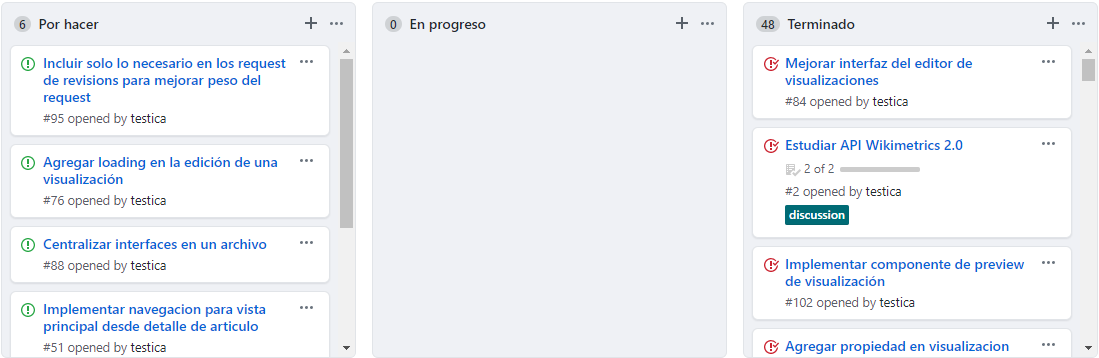
\includegraphics[scale=0.4]{images/marco_aplicativo/github_board.png}
    \captionof{figure}{Pizarra de Github}
    \label{fig:githubBoard}
    \bigbreak
\end{center}

La pizarra de Github, véase la \textbf{Figura \ref{fig:githubBoard}}, es una herramienta de la metodología Kanban \cite{BookKanban}, en donde visualizar el flujo de trabajo y hacerlo visible es la base para comprender cómo avanza el trabajo. Sin comprender el flujo de trabajo, realizar los cambios adecuados es más difícil. Una forma común de visualizar el flujo de trabajo es el uso de columnas. Las columnas representan los diferentes estados o pasos en el flujo de trabajo. Kanban logra un desarrollo evolutivo e incremental, donde las soluciones de las asignaciones puede que no sean las mejores comenzando, pero a medida que se itera se va perfeccionando.

\section{Realización de tareas}
A continuación, de listarán las tareas de mayor relevancia ordenadas cronológicamente, con la descripción del problema y el resultado.

\begin{enumerate}
  \smallbreak
  \item\textbf{Preparar entorno de desarrollo}
  \smallbreak

  Antes de empezar el desarrollo se necesita instalar o preparar el ambiente para el uso de las herramientas:
  \begin{itemize}
      \item Instalar Node\footnote{\url{https://nodejs.org}} para servir la aplicación web local.
      \item Instalar NPM\footnote{\url{https://www.npmjs.com/}} (Node Package Manager) necesaria para instalar paquetes JavaScript como Angular y dependencias.
      \item Instalar editor de texto inteligente, en preferencia personal, Visual Studio Code.
      \item Instalar navegadores modernos, principalmente Google Chrome y Firefox, para reproducir la aplicación web y asegurar el soporte de la misma.
  \end{itemize}

  \smallbreak
  \item\textbf{Elaborar estructura base de la aplicación}
  \smallbreak
  Lo principal es tener la estructura base del proyecto en código y tener la configuración del framework Angular lista.
  
  Afortunadamente, existe una herramienta llamada \textbf{angular-cli}, que facilita la creación de un proyecto en Angular poniendo lo siguiente en el terminal:
  \begin{minted}[linenos]{console}
    # instalar angular-cli
    npm install -g @angular/cli
    # crear proyecto
    ng new wiki-history-client
  \end{minted}

  \smallbreak
  \item\textbf{Investigar API de WikiMedia}
  \smallbreak
  
  Es necesario ofrecer los artículos del \textit{watchlist} de los usuarios para que posteriormente puedan analizarlos con la aplicación, dado esto se necesita saber cómo autenticar un usuario y obtener su \textit{watchlist} haciendo uso del API.
  
  En el momento cuando se desempeñó esta tarea hubo un problema con el API de autenticación, debido a que estaban abandonando la manera tradicional y migrando a una más segura usando OAuth2\footnote{\url{https://oauth.net/2/}}, por motivos de privilegios no fue posible registrar la aplicación con el método nuevo de autenticación.
  
  Debido a esto, no iba a ser posible extraer el \textit{watchlist} sin credenciales de usuarios, por lo que se optó la decisión de construir un API propia donde se gestionaran usuarios y ellos manualmente agregarían los artículos de interés.
  
  \smallbreak
  \item\textbf{Implementar vista de Artículos}
  \smallbreak
  
  La vista principal de la aplicación sería una lista de artículos de interés.
  
  En la versión actual, los datos de los artículos se simularon en una variable, para probar que la vista funcionaba.
  \begin{center}
      \bigbreak
      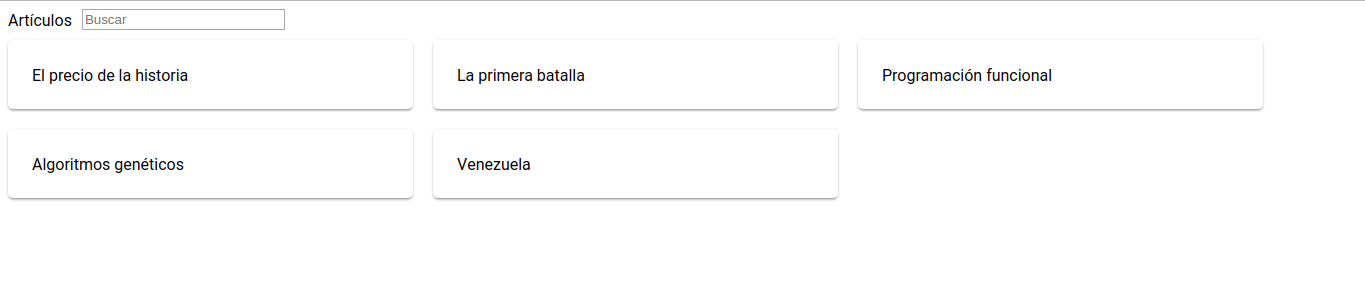
\includegraphics[scale=0.2]{images/marco_aplicativo/lista_articulos.png}
      \captionof{figure}{Lista de artículos}
      \label{fig:article_list}
      \bigbreak
  \end{center}
  
  Se usó un elemento de Angular Material llamado md-card, para formar el estilo de un artículo. La propiedad *ngFor es una directiva de angular que nos permite replicar ese elemento tanta veces como iteraciones tenga. Además hacemos uso de fxFlex que nos permite ajustar el tamaño del elemento dependiendo de las dimensiones de la pantalla, véase en la \textbf{Figura \ref{fig:article_list}} el resultado.
  \begin{minted}[linenos]{html}
    <md-card 
        *ngFor="let article of articles"
        fxFlex="30" fxFlex.sm="50" fxFlex.xs="100">
        {{article.title}}
    </md-card>
  \end{minted}
  
  \smallbreak
  \item\textbf{Implementar vista de detalle de  Artículo}
  \smallbreak
  
  Al presionar un artículo de la lista nos tiene que  dirigir a un detalle para acceder a más información del mismo.
  
  En la versión actual simplemente se mostrará una vista blanca que representa el detalle. De esta forma, se programó que al pisar un artículo direccione a la vista del detalle. La ruta del detalle se representa por: 
  \begin{minted}{console}
   /articles/<titulo_artículo>
  \end{minted}
  
  \smallbreak
  \item\textbf{Implementar servicio (API) para manejar usuarios y configuraciones}
  \smallbreak
  
  Es necesario un servicio que delegue la autenticación y gestión de los recursos persistentes como usuarios y artículos.
  
  Se desarrolló un API usando el micro framework Python Flask\footnote{\url{flask.pocoo.org/}} y para la persistencia de los datos se usó MongoDB, se consideró una base de datos NoSQL debido a que los datos no están relacionados, son simplemente usuarios con configuraciones personales.
  
  Se implementaron las siguientes rutas en el API:
  \begin{minted}{console}
   POST /sign-up
   POST /sign-in
   GET /articles
   POST /articles
   DELETE /articles/<titulo>
  \end{minted}
  
  Para la autorización de recursos, se usó el mecanismo JWT\footnote{\url{https://jwt.io/}}(JSON Web Token), que consiste en la generación de un token resultado de datos cifrado con una clave privada. De esta forma podemos extraer del token el usuario y corroborar si la solicitud del recurso es válida.
  
  
  En la versión actual, el modelo de cada usuario se verá representado de la siguiente manera:
  
  \begin{minted}{json}
  {
    "username": "admin",
    "password": "202cb962ac59075b964b07152d234b70",
    "articles": [
        {
         "title": "Titulo 1",
         "locale": "es"
        }
    ]
  }
  \end{minted}
  
  Es importante acotar que las contraseñas son almacenadas usando la función hash MD5\footnote{\url{https://en.wikipedia.org/wiki/MD5}}.

  \smallbreak
  \item\textbf{Agregar documentación y dependecias de API}
  \smallbreak
  
  A nivel de desarrollo es importante tener instrucciones de cómo hacer funcionar las cosas por si otro desarrollador continúa el trabajo, dado esto, se le agrego documentación y se fijaron las versiones de las dependencias para hacerla funcionar en cualquier momento.
  
  \smallbreak
  \item\textbf{Implementar vista para iniciar sesión}
  \smallbreak
  
  Se requiere una vista para poder iniciar sesión con un usuario y contraseña.
  
  Se implementó un formulario pidiendo ambos requerimientos, que puede ser accedido bajo la ruta:
  \begin{minted}{console}
   /sign-in
  \end{minted}
  
  Se creó un servicio de Angular para abstraer la comunicación con el API para hacer el inicio de sesión:
  \begin{minted}[linenos]{ts}
    import { Injectable } from '@angular/core';
    import { Http } from '@angular/http';
    import { environment } from '../environments/environment';
    import { ISignIn } from './resource';
    
    @Injectable()
    export class AuthService {
    
      private loggedIn = false;
    
      constructor(private http: Http) {
        this.loggedIn = !!window.localStorage.getItem('auth_token');
      }
    
      signIn(username: string, password: string) {
        return this.http.post(
        `${environment.API_URL}/sign-in`,
         {username, password}
         )
        .toPromise()
        .then(res => {
          const obj: ISignIn = res.json();
          // store token
          window.localStorage.setItem('auth_token', obj.access_token);
          return obj;
        });
      }
    
    }
  \end{minted}
  
  Un servicio es una instancia \textit{singleton}, que puede ser inyectada y usada en cualquier parte de la aplicación, luego de crear el servicio podemos hacer inicio de sesión con:
  \begin{minted}[linenos]{ts}
  signIn("admin","1234").then();
  \end{minted}

  \smallbreak
  \item\textbf{Implementar vista para registrar un usuario}
  \smallbreak
  
  Es indispensable poder registrar un usuario para luego poder acceder a él.
  
  Por lo tanto, se creó la vista usando un componente que proyecta un formulario similar al iniciar sesión.
  
  \smallbreak
  \item\textbf{Implementar componente de sugerencia de artículos de Wikipedia}
  \smallbreak
  
  Una vez creado un usuario, lo siguiente es preparar los artículos que queremos examinar. Como no hay forma de obtener el watchlist se tiene que ofrecerle una manera de buscar los artículos de Wikipedia a desear.
  
  Se implementó un input que sugiere artículos de Wikipedia a medida que escribes cualquier texto, además se consideró el idioma, véase la \textbf{Figura \ref{fig:sugerencia_wikipedia}}.
  
  \begin{center}
      \bigbreak
      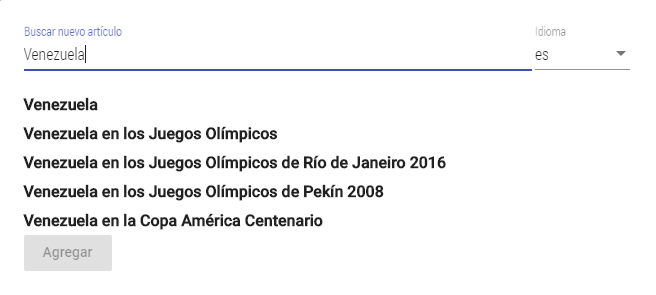
\includegraphics[scale=0.6]{images/marco_aplicativo/sugerencia_wikipedia.png}
      \captionof{figure}{Caja de sugerencias de artículos de Wikipedia}
      \label{fig:sugerencia_wikipedia}
      \bigbreak
  \end{center} 
  
  \smallbreak
  \item\textbf{Implementar componente y servicio para agregar artículo}
  \smallbreak
  
  Surge la necesidad de persistir los artículos agregados por los usuarios, por lo que se tiene que habilitar la opción para crear artículos y extraerlo asíncronamente usando el API de Wikimetrics 2.0.
  
  Se abstrae la petición al API para crear un artículo a través de un servicio, y se encapsula el componente de la tarea anterior en otro componente que interactué con el servicio, véase la \textbf{Figura \ref{fig:nuevo_articulo_flujo}}.
  
  \begin{center}
      \bigbreak
      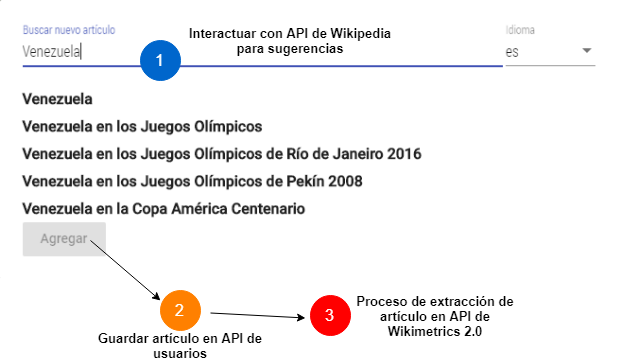
\includegraphics[scale=0.5]{images/marco_aplicativo/nuevo_articulo_flujo.png}
      \captionof{figure}{Flujo del agregar artículo. En el punto (1) se accede al API de Wikipedia para obtener los artículos sugeridos, luego al presionar agregar sucede el punto (2) que hace un request al API nuestra de usuarios para agregar el artículo y luego en el punto (3) se hace un request en el API de Wikimetrics 2.0 para activar el proceso de extracción del artículo}
      \label{fig:nuevo_articulo_flujo}
      \bigbreak
  \end{center} 
  
  \smallbreak
  \item\textbf{Implementar servicio para obtener lista de artículos}
  \smallbreak
  
  Para la versión actual, se estaba trabajado con una lista de artículos falsa. Por lo tanto surge la necesidad de poder pedir la lista real de artículos asociada a un usuario.
 
  Se implementa un servicio que abstrae la lógica de realizar la petición a la ruta para pedir los artículos.
  
  \smallbreak
  \item\textbf{Crear componente dedicado para los artículos en el listado}
  \smallbreak
  
  El estilo de los artículos en el listado es hasta ahora muy simple y vacío.
 
  Se encapsula la lógica de la carta de un artículo en un componente, para abstraer funcionalidades complejas y se muestra más información del mismo, con un mejor estilo.
  
  \smallbreak
  \item\textbf{Actualizar estado del artículo cada cierto tiempo}
  \smallbreak
  
  Se sabe que se tiene que hacer un proceso de extracción del artículo para que el API de Wikimetrics pueda ofrecer datos a visualizar, pero actualmente no se tiene forma de saber si el artículo ya fue extraído o no, de alguna forma se tiene que comunicar esa información al usuario para que esté al tanto del proceso. Un artículo puede tardar varios minutos en extraerse, todo esto depende del tamaño y cantidad de ediciones.
 
  Cuando un artículo es mandado a extraer, este responde con un código que nos servirá para preguntar por su estado. Replicamos esta lógica en el lado del API de usuarios, guardando el código y su estado actual:
  \begin{minted}[linenos]{json}
     {
        "locale": "es",
        "extract": {
            "status": "pending",
            "id": "665d387e-e547-4275-8abf-1076eacf8f92"
        },
        "title": "Universidad Central de Venezuela"
    }
  \end{minted}
  
  El proceso de extracción puede pasar por 4 estados: \textit{pending} (\textbf{Figura \ref{fig:article_pending}}), \textit{success} (\textbf{Figura \ref{fig:article_success}}), \textit{failure}, \textit{in progress}.
  
  Para dar una interacción mas precisa al usuario, cada 10 segundos se hace un request para comprobar el estado y se actualiza en nuestra API, la condición de parada es que este \textit{success} o \textit{failure}
  
  \begin{center}
      \bigbreak
      
\includegraphics{images/marco_aplicativo/article_pending.png}
      \captionof{figure}{Estilo de un artículo en estado pendiente de extracción}
      \label{fig:article_pending}
      \bigbreak
  \end{center}
  \begin{center}
      \bigbreak
      
\includegraphics{images/marco_aplicativo/article_extracted.png}
      \captionof{figure}{Estilo de un artículo en estado exitoso de extracción}
      \label{fig:article_success}
      \bigbreak
  \end{center} 
  
  \smallbreak
  \item\textbf{Manejar autorización en las vistas}
  \smallbreak
  
  Hasta este punto del desarrollo no hay ningún método que proteja las vistas que requieran autenticación, es decir anteriormente se puede intentar acceder a la vista del listado de artículos sin haber iniciado sesión, queda claro que al entrar a esta vista la petición daría error por seguridad del API.
  
  Se agrega una capa más de seguridad a nivel de cliente, para que el usuario no puede entrar sin autenticación a dichas vistas. Para esto usaremos guardias de rutas, a continuación la definición del guardia:
  \begin{minted}[linenos]{ts}
    import { Injectable } from '@angular/core';
    import { CanActivate, Router } from '@angular/router';
    import { AuthService } from './auth.service';
    
    @Injectable()
    export class AuthGuard implements CanActivate {
    
      constructor(
        private authSvc: AuthService,
        private router: Router) {}
    
      canActivate() {
        if (!this.authSvc.isSigned()) {
          this.router.navigate(['/sign-in']);
        }
    
        return this.authSvc.isSigned();
      }
    }
  \end{minted}
  
  Podemos observar que antes de navegar a una ruta la función \textbf{canActivate()} se llamará, esto verifica si hay una sesión de usuario válida, en caso contrario redirige al inicio de sesión.
  
  \smallbreak
  \item\textbf{Implementar barra superior (navbar)}
  \smallbreak

  Es importante desplegar una barra superior que muestre información extra y despliegue acciones, principalmente navegación a vista principal y cerrar sesión.
  
  
  Se implementó un componente para la barra y un servicio para cambiar sus configuraciones, como título, acciones y cierre de sesión, véase la \textbf{Figura \ref{fig:navbar}}.
  
  \begin{center}
      \bigbreak
      
\includegraphics[scale=0.6]{images/marco_aplicativo/navbar.png}
      \captionof{figure}{Barra superior}
      \label{fig:navbar}
      \bigbreak
  \end{center} 
  
  \smallbreak
  \item\textbf{Implementar ruta en API para obtener un artículo en especifico:}
  \smallbreak

  Al entrar al detalle de un artículo se necesita solicitar la información de ese artículo en particular.
  
  Se implementó en API la nueva ruta:
  \begin{minted}{console}
   GET /articles/<idioma>/título
  \end{minted}
  
  Luego se adapta al componente del detalle de artículo.
  
  \smallbreak
  \item\textbf{Implementar servicio para pedir información sobre revisiones de un artículo}
  \smallbreak

  En el detalle de artículo se mostrará cierta información básica sobre las ediciones, como el número total de ediciones y las últimas 20.
  
  Para tener el número total de ediciones se tiene que hacer uso de una ruta que Wikimetrics provee:
  
  \begin{minted}{console}
   GET /api/v1/count?locale=en&title=Venezuela
  \end{minted}
  
  Para tener la información de las últimas 20 ediciones ordenadas por fecha descendientemente:
  \begin{minted}{console}
   GET /api/v1/revisions?locale=en&title=Venezuela
   &page_size=20&sort=desc
  \end{minted}
  
  Se encapsularon en el servicio de wikimetrics para abstraer su uso.
  
  \smallbreak
  \item\textbf{Implementar componente de visualización}
  \smallbreak

  Algo sumamente importante es la posibilidad de desplegar gráficas, en distintos casos, la aplicación necesitará de un componente que muestre gráficas variables.
  
  Se abstraerá la visualización de un gráfica en un componente, apoyándose de la biblioteca Plotly. El componente acepta las siguientes entradas para variar su configuración:
  
  \begin{minted}[linenos]{ts}
  @Input() chartType: 'pie' | 'bar' | 'scatter'
    | 'scattergl' | 'line' | 'area';
  @Input() chartX: string[] | number[];
  @Input() chartY: string[] | number[];
  @Input() chartXTitle = '';
  @Input() chartYTitle = '';
  @Input() chartTitle = '';
  \end{minted}
  
  En donde \textbf{chartType} es para pasarle el tipo de gráfica que queremos desplegar, \textbf{chartX} y \textbf{chartY} correponde el set de datos para ambos ejes, \textbf{chartXTitle} y \textbf{chartYTitle} describe el título de ambos ejes y \textbf{chartTitle} hace referencia al título de la visualización.
  
  
  Se consideró hacer el componente de tal forma que fuera reactivo al cambio dimensión de la pantalla, es decir, las visualizaciones son \textit{responsive}.
  
  \begin{minted}[linenos]{ts}
  this.resizeService.onResize$.subscribe(() =>
    Plotly.Plots.resize(this.gd)
  );
  \end{minted}
  
  Haciendo uso del patrón \textit{observer}, con ayuda de la biblioteca ReactiveX \footnote{\url{http://reactivex.io/}}, cada vez que la pantalla cambia su posición se notifica mediante un servicio y se ajusta el tamaño de la visualización.
  
  \smallbreak
  \item\textbf{Mostrar información específica en el detalle del artículo}
  \smallbreak

  Al entrar al detalle del artículo hay que que encontrar información específica y que sume valor.
  
  Por lo tanto, se considera colocar el número de ediciones, fecha de última edición, autor de la última edición, tamaño del artículo y una visualización que considere el tamaño y fecha de las ultimas 20 ediciones, véase la \textbf{Figura \ref{fig:article_detail_main}}.
  
  \begin{center}
      \bigbreak
      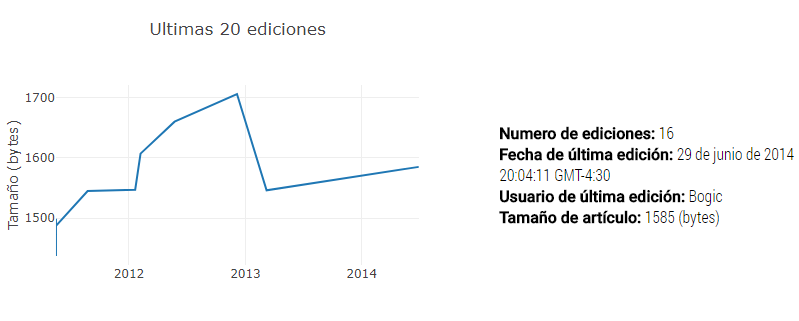
\includegraphics[scale=0.5]{images/marco_aplicativo/article_detail_main.png}
      \captionof{figure}{Visualización e información específica del artículo}
      \label{fig:article_detail_main}
      \bigbreak
  \end{center}
  
  De la siguiente manera quedaría el código para mostrar la gráfica, haciendo uso del componente de visualización :
  \begin{minted}[linenos]{html}
  <app-visualization
    chartTitle="Ultimas 20 ediciones"
    chartYTitle="Tamaño (bytes)"
    chartType="scatter"
    [chartX]="timestamps(revisions)"
    [chartY]="sizes(revisions)" 
    fxFlex="60" fxLayout="column">
  </app-visualization>
  \end{minted}
  
  Las función \textbf{timestamps(revisions)} extrae la fecha de edición y la función \textbf{sizes(revisions)} extrae el tamaño de cada edición
  
  \smallbreak
  \item\textbf{Implementar gráfica WikiHistoryFlow}
  \smallbreak

  A nivel de visualizaciones, ofrecer la gráfica WikiHistoryFlow era un requerimiento principal. Con esta gráfica se puede identificar el comportamiento de un usuario, el estado del artículo en el tiempo y detectar patrones de vandalismo.
  
  La visualización proviene principalmente de la herramienta de History Flow Visualization \cite{HistoryFlow}, que consta de barras laterales, donde cada barra representa una edición. La altura de la barra representa el tamaño, el color representa un usuario único y el ancho representa la distancia del texto del artículo de la versión anterior y la actual, véase la \textbf{Figura \ref{fig:history_flow}} y \textbf{Figura \ref{fig:history_flow_original}}.
  
  \begin{center}
      \bigbreak
      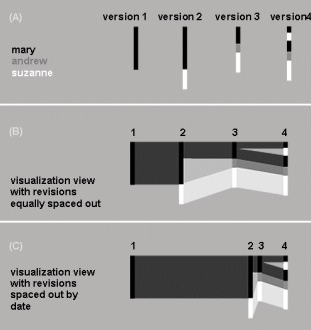
\includegraphics{images/marco_aplicativo/history_flow1.png}
      \captionof{figure}{Explicación del mecanismo usado en la visualización de History Flow}
      \label{fig:history_flow}
      \bigbreak
  \end{center}
  
  \begin{center}
      \bigbreak
      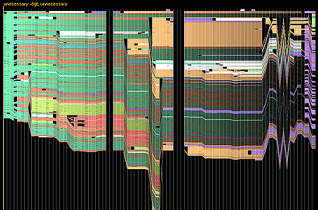
\includegraphics{images/marco_aplicativo/history_flow_original.png}
      \captionof{figure}{Herramienta History Flow Visualization}
      \label{fig:history_flow_original}
      \bigbreak
  \end{center}
  
  Para este trabajo por motivos de cómputos, se adaptara la visualización a una versión más simple, llamada History Graph \cite{HistoryGraph}, véase la \textbf{Figura \ref{fig:history_graph}}.
  
  \begin{center}
      \bigbreak
      
\includegraphics{images/marco_aplicativo/history_graph.png}
      \captionof{figure}{Visualización History Graph}
      \label{fig:history_graph}
      \bigbreak
  \end{center}
  
  No hay manera de desplegar esta gráfica con la biblioteca Plotly dado que es bastante específica, por lo tanto para este caso se optó por la biblioteca D3 que nos permite libertad a la hora de construir visualizaciones.
  
  Se encapsuló la visualización en un componente, en donde la primera tarea fue ordenar las ediciones por orden de creación de manera cronológica, luego se almacenó el valor de tamaño de edición máximo y se declaró un arreglo que contiene la distancia de cada edición contra la anterior (se asigno 0 para la primera edición). Para calcular la distancia entre dos textos se usó una biblioteca que aplica la distancia de Levenshtein.
  
  Calculados los datos anteriores se tiene todo listo para graficar, en donde cada elemento del arreglo de revisiones ordenado cronológicamente representa una barra usando el elemento \textbf{div} de html.
  
  \begin{minted}[linenos]{ts}
    d3.select(this.elemRef.nativeElement)
    .selectAll('div.bar')
    .data(revsOrderByDate)
    .enter().append('div').attr('class', 'bar')
  \end{minted} 
  
  Para asignar el ancho, se usó del arreglo de distancias antes calculado. Adicionalmente, se tiene que conservar el tamaño de manera proporcional a la pantalla, por lo que se le asigno a cada barra un ancho base predeterminado. Para que no ocurrieran desbordamiento de píxeles se uso una función de CSS llamada \textbf{calc} para ajustar el ancho base mas la distancia.
  
  \begin{minted}[linenos]{ts}
   .style('width', (_, i) => `calc(
    ${((1 / totalRev) * 100)}% + ${distanceRevs[i]}px
    )`
   )
  \end{minted} 
  
  Para asignar el alto basta con dividir el tamaño de la edición entre el tamaño máximo anteriormente calculado.
  
  \begin{minted}[linenos]{ts}
   .style('height', rev => `${(rev.size / maxSize) * 100}%`)
  \end{minted} 
  
  Finalmente, para asignar el color de la barra se usó una función hash que recibe un nombre de usuario (string) y retorna un color hexadecimal.
 
  \begin{minted}[linenos]{ts}
  .style('background', rev => 
    `${this.stringToColour(rev.user)}`
    )
  \end{minted}
  
  \begin{minted}[linenos]{ts}
  stringToColour(str: string) {
    let hash = 0;
    for (let i = 0; i < str.length; i ++) {
      // tslint:disable-next-line:no-bitwise
      hash = str.charCodeAt(i) + ((hash << 5) - hash);
    }
    let colour = '#';
    for (let i = 0; i < 3; i ++) {
      // tslint:disable-next-line:no-bitwise
      const value = (hash >> (i * 8)) & 0xFF;
      colour += ('00' + value.toString(16)).substr(-2);
    }
    return colour;
  }
  \end{minted} 
  
  Como funcionalidad adicional, se agregó un \textit{tooltip} que muestra nombre del usuario, fecha y tamaño de la edición cuando nos apoyamos sobre cualquier barra, véase la \textbf{Figura \ref{fig:wiki_history_flow}}.
  
  \begin{center}
      \bigbreak
      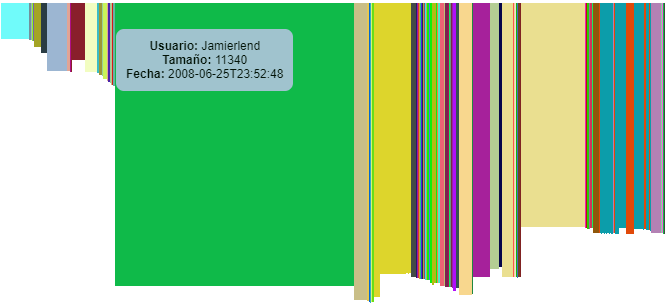
\includegraphics[scale=0.6]{images/marco_aplicativo/wiki_history_flow.png}
      \captionof{figure}{Visualización Wiki History Flow del artículo 'Programación dirigida por eventos'}
      \label{fig:wiki_history_flow}
      \bigbreak
  \end{center}
  
  
  \smallbreak
  \item\textbf{Agregar enlace a wikipedia del artículo}
  \smallbreak

  En el detalle del artículo pude ser de gran utilidad tener un enlace que dirija al artículo en Wikipedia, véase la \textbf{Figura \ref{fig:article_detail_link}}.
  
  \begin{center}
      \bigbreak
      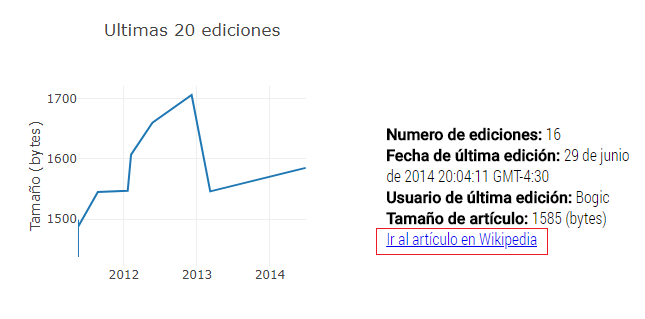
\includegraphics[scale=0.6]{images/marco_aplicativo/article_detail_main_with_link.png}
      \captionof{figure}{Información principal de detalle de artículo incluyendo vínculo a Wikipedia}
      \label{fig:article_detail_link}
      \bigbreak
  \end{center}
  
  \smallbreak
  \item\textbf{Implementar componente y servicio para crear nueva visualización}
  \smallbreak

  Un requerimiento principal es poder crear nuestras visualizaciones sobre un artículo y poder editarlas, pero como primer paso necesitamos la creación de la misma preguntando información básica.
  
 
  Se posicionó un botón en la barra de navegación capaz de crear la visualización. Al pisarse mostrará un dialogo preguntando el título y descripción que tendrá la visualización, véase la \textbf{Figura \ref{fig:create_vis_main}}.

  \begin{center}
      \bigbreak
      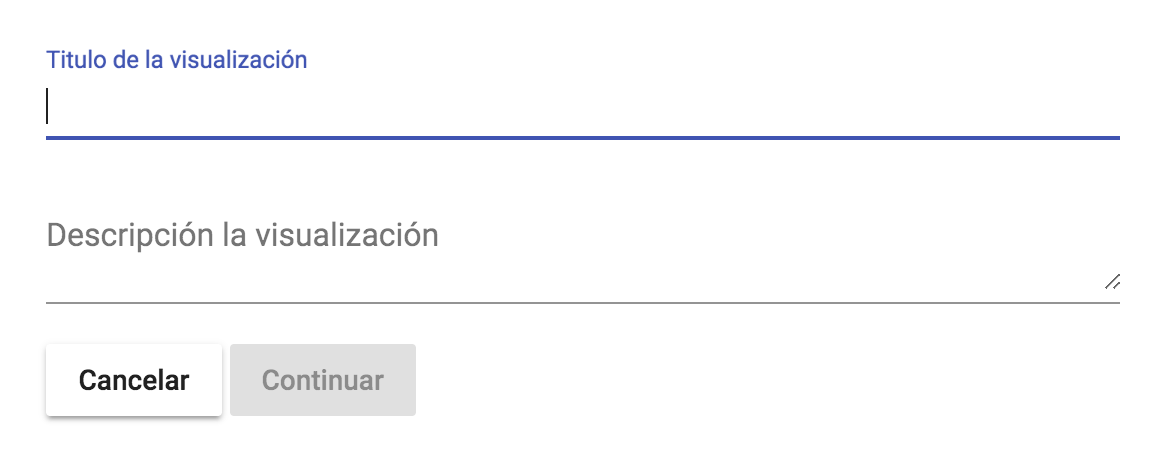
\includegraphics[scale=0.55]{images/marco_aplicativo/create_vis_main.png}
      \captionof{figure}{Información principal para crear una visualización}
      \label{fig:create_vis_main}
      \bigbreak
  \end{center}
  
  Dado esto, se manejó en base de datos un objeto de visualizaciones donde internamente cada visualización es referenciada por el título:

  \begin{minted}[linenos]{json}
   {
    "title": "Universidad Central de Venezuela",
    "visualizations": {
        "Visualización de usuarios": {
            "query": "",
            "type": "",
            "description": "Torta"
        },
        "Visualización de ediciones menores": {
            "query": "",
            "type": "",
            "description": ""
        }
    }
   }
  \end{minted}
  
  \smallbreak
  \item\textbf{Implementar componente y servicio para crear nueva visualización}
  \smallbreak

  Es necesario listar las visualizaciones creadas en el detalle de artículo, para luego ser accedidas.
 
  Se crearon dos listas, una de las visualizaciones creadas por el usuario y otra de visualizaciones predefinidas por la aplicación.
  
  \smallbreak
  \item\textbf{Implementar componente para seleccionar el query de la visualización}
  \smallbreak

  Creada una visualización es necesario empezar a editarla para construir la gráfica respectiva, por lo que necesitamos ofrecer la herramienta para seleccionar lo que se desear visualizar.
  
  La herramienta constará de tres (3) selectores, el primero permite filtrar, el segundo ofrece operaciones de agrupaciones y el tercero permite agrupar, véase la \textbf{Figura \ref{fig:query_selector}}.
  
  El selector de \textbf{filtro} ofrece filtrar por edición anónima, tamaño de la edición, id de usuario, nombre de usuario, edición menor y fecha de edición.
  
  El selector de \textbf{vista} ofrece operadores sobre agrupaciones como contar, sumar tamaño de ediciones, promediar tamaño de ediciones, máximo tamaño de ediciones y mínimo tamaño de ediciones.
  
  El selector de \textbf{agrupar} ofrece la posibilidad de agrupar según edición anónima, id de edición, tamaño de edición, id de usuario, nombre de usuario, edición menor, fecha (mes), fecha (mes y año), fecha (día, mes y año).
  
  
  \begin{center}
      \bigbreak
      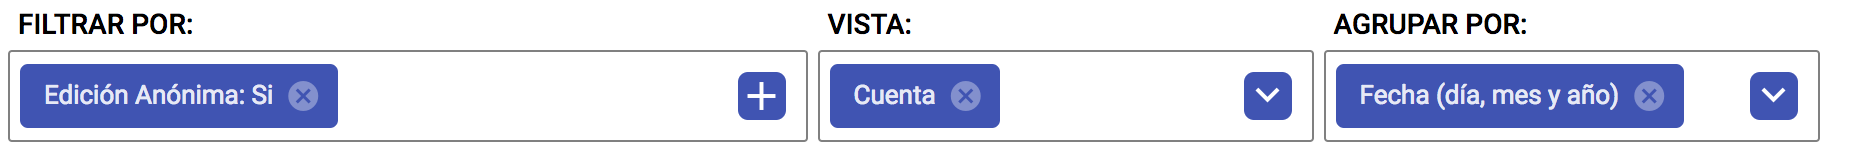
\includegraphics[scale=0.3]{images/marco_aplicativo/query_selector.png}
      \captionof{figure}{Vista de componente para seleccionar query de la visualización}
      \label{fig:query_selector}
      \bigbreak
  \end{center}
  
  El valor de cada opción de los selectores referencia la parte del query de MongoDB necesario. Por lo tanto se realizó una función para construir el query final a enviar al API de Wikimetrics:
  
  \begin{minted}[linenos]{ts}
  buildQuery(): WikimetricsQuery[] {
    // setup filters
    let obj = {};
    this.selectedFilters.forEach(i => {
      obj = merge(obj, i.value);
    });

    // build query
    const newQuery = [
      {
        $match: obj
      },
      {
        $group: {
          _id: this.selectedGroup ?
          this.selectedGroup.value : null ,
          ... this.selectedView && this.selectedView.value ?
          { result: this.selectedView.value } : {}
        }
      }
    ];

    return newQuery;
  }
  \end{minted}
  
  En donde \textbf{obj} es el objeto con todos los filtros, \textbf{selectedGroup.value} el campo u objeto de la agrupación y \textbf{selectedView.value} el nombre del operador de agrupaciones.
  
  Por último, si se tiene un query formado, se necesita la función inversa que sería extraer del query los valores para rellenar los selectores. Esta funcionalidad es extensa por lo que se puede revisar en el código fuente del proyecto en el componente \textbf{query-selector.component.ts}.
  
  \smallbreak
  \item\textbf{Implementar componente para editar visualizaciones}
  \smallbreak

  Cuando se obtiene la respuesta del query, se tiene los datos pero no listos para visualizarlos, tiene que darse un formato entendible para usarlo con el componente de visualización anteriormente creado, además se tiene que definir el tipo de visualización a mostrar.
  
  
  Se tuvo que condicionar cada uno de los casos posibles de las opciones, en el caso de edición menor, interpretar a 'No menor' y 'Menor', para usuario anónimo se interpretó como 'Anónimo' y 'No Anónimo'. En el caso de agrupación por fecha se usó la biblioteca luxon\footnote{\url{https://moment.github.io/luxon/}} (alternativa ligera de Momentjs) para darle un mejor formato, véase la \textbf{Figura \ref{fig:edit_vis}}.
  
  
  \begin{center}
      \bigbreak
      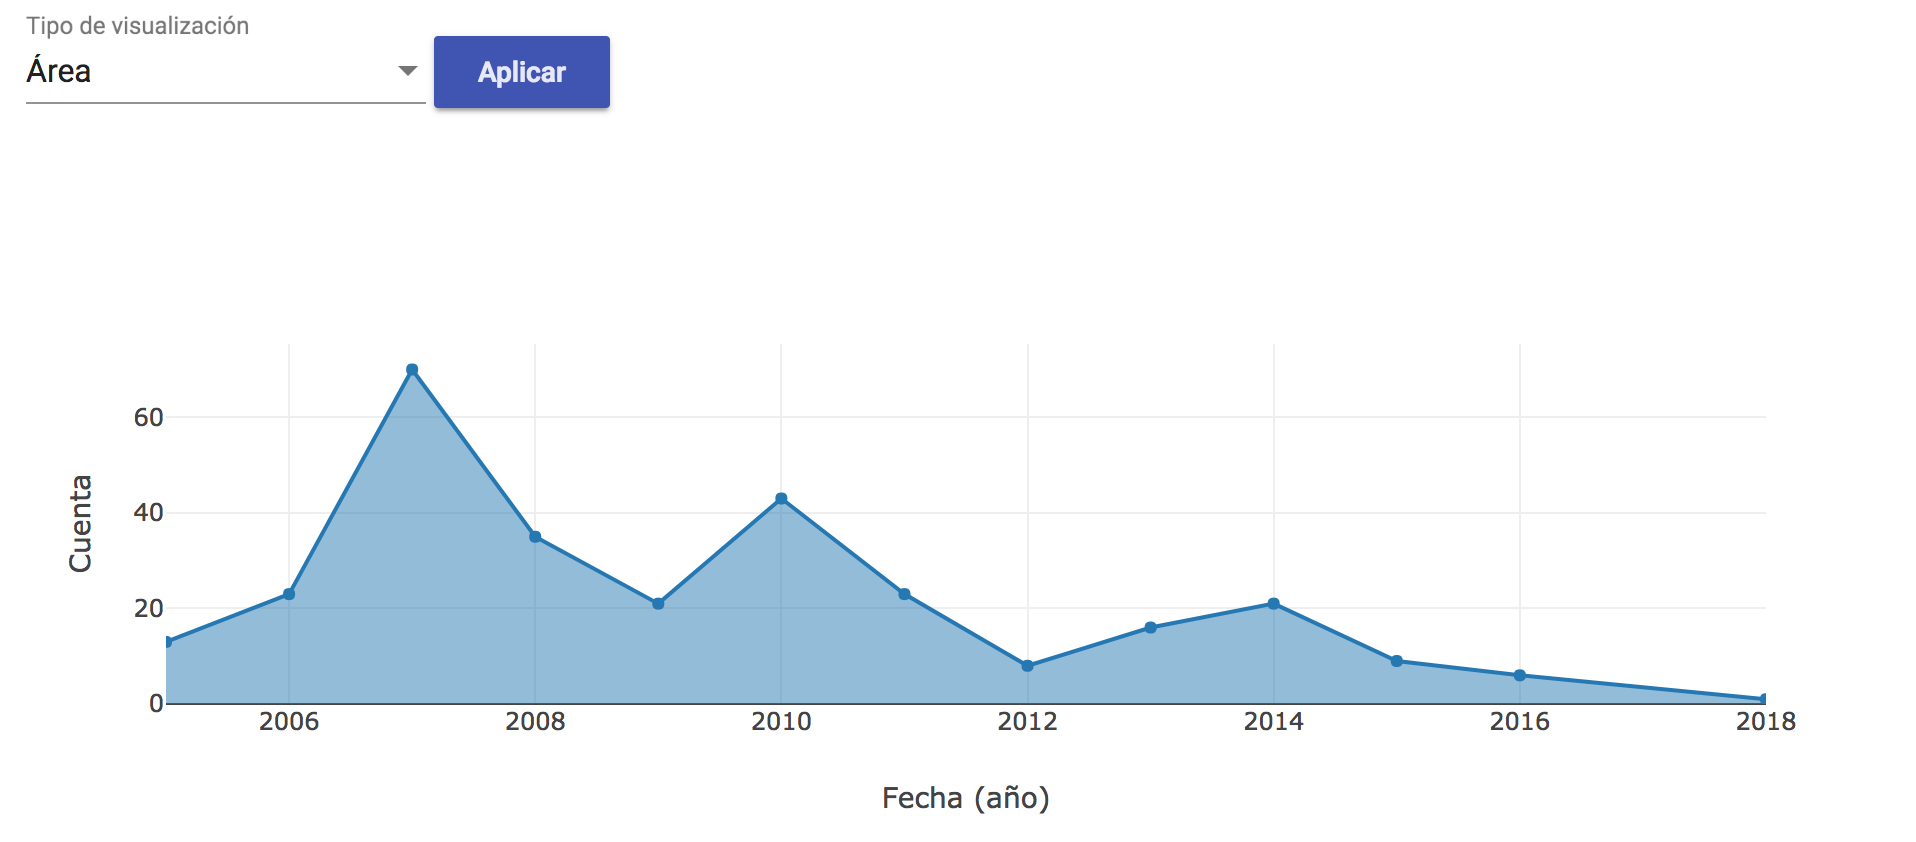
\includegraphics[scale=0.35]{images/marco_aplicativo/edit_vis.png}
      \captionof{figure}{Componente de visualización y selector de tipo en el editor de visualizaciones}
      \label{fig:edit_vis}
      \bigbreak
  \end{center}
  
  El selector de tipo visualizaciones ofrece las siguientes opciones:
  \begin{itemize}
    \item\textbf{Número}: muestra un número total, solo es válido cuando no se aplica agrupación, véase la \textbf{Figura \ref{fig:vis_number}}.
    
        \begin{center}
          \bigbreak
          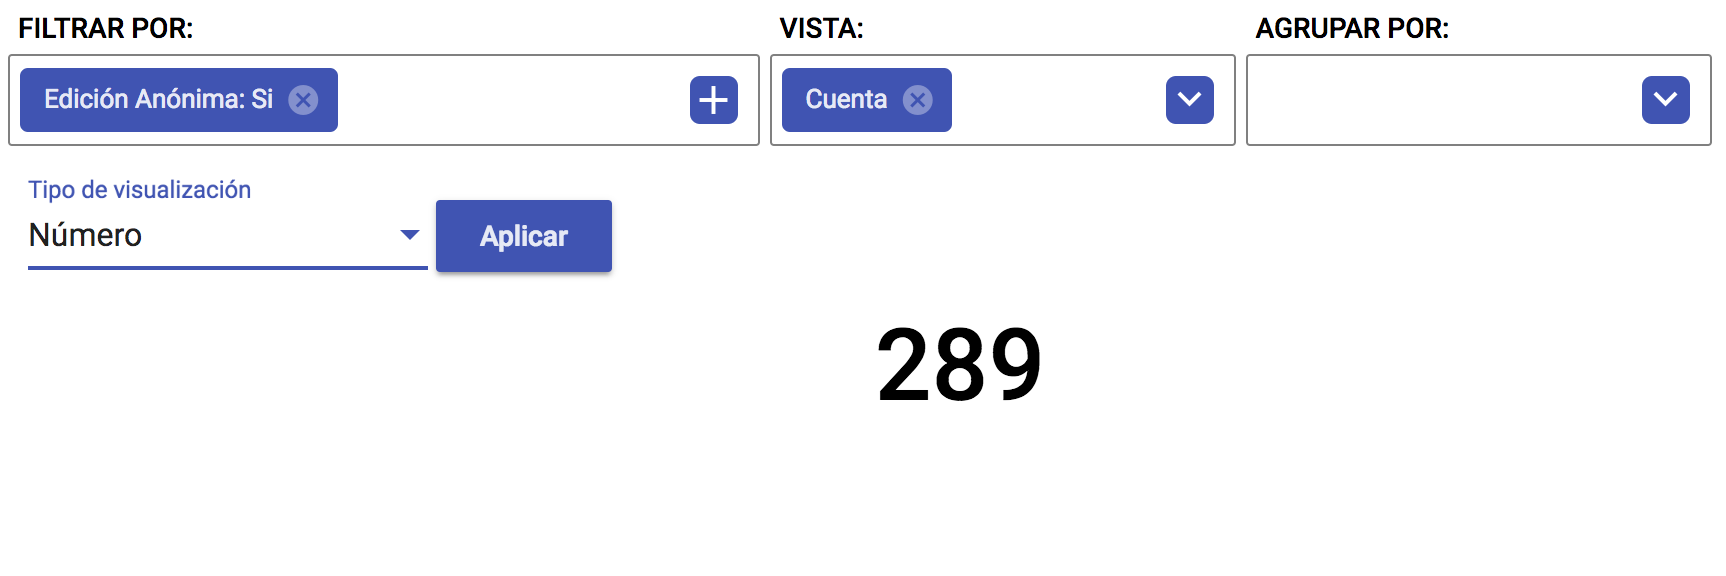
\includegraphics[scale=0.35]{images/marco_aplicativo/vis_number.png}
          \captionof{figure}{Visualización tipo número}
          \label{fig:vis_number}
          \bigbreak
        \end{center}

    \item\textbf{Línea}: gráfica que consiste en trazar un línea entre cada par de puntos, véase la \textbf{Figura \ref{fig:vis_line}}.
        \begin{center}
          \bigbreak
          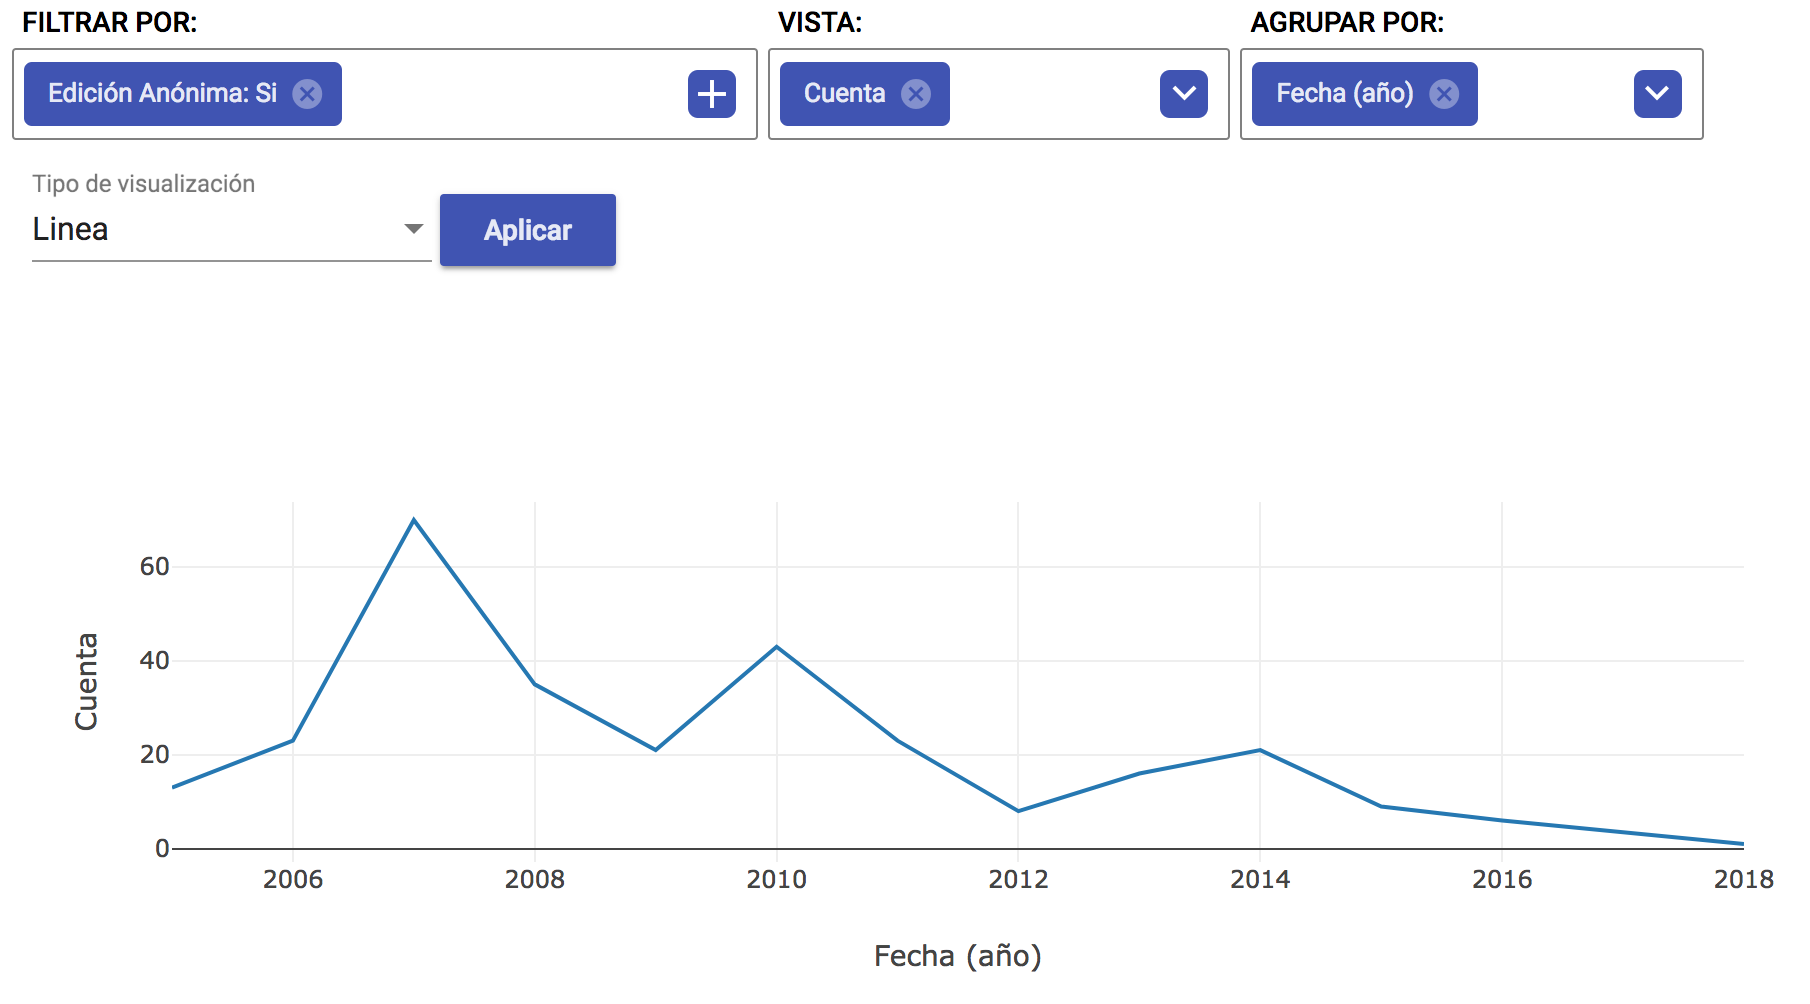
\includegraphics[scale=0.35]{images/marco_aplicativo/vis_line.png}
          \captionof{figure}{Visualización tipo línea}
          \label{fig:vis_line}
          \bigbreak
        \end{center}

    \item\textbf{Barra}: gráfica que consiste en proyectar barras, véase la \textbf{Figura \ref{fig:vis_bar}}.
        \begin{center}
          \bigbreak
          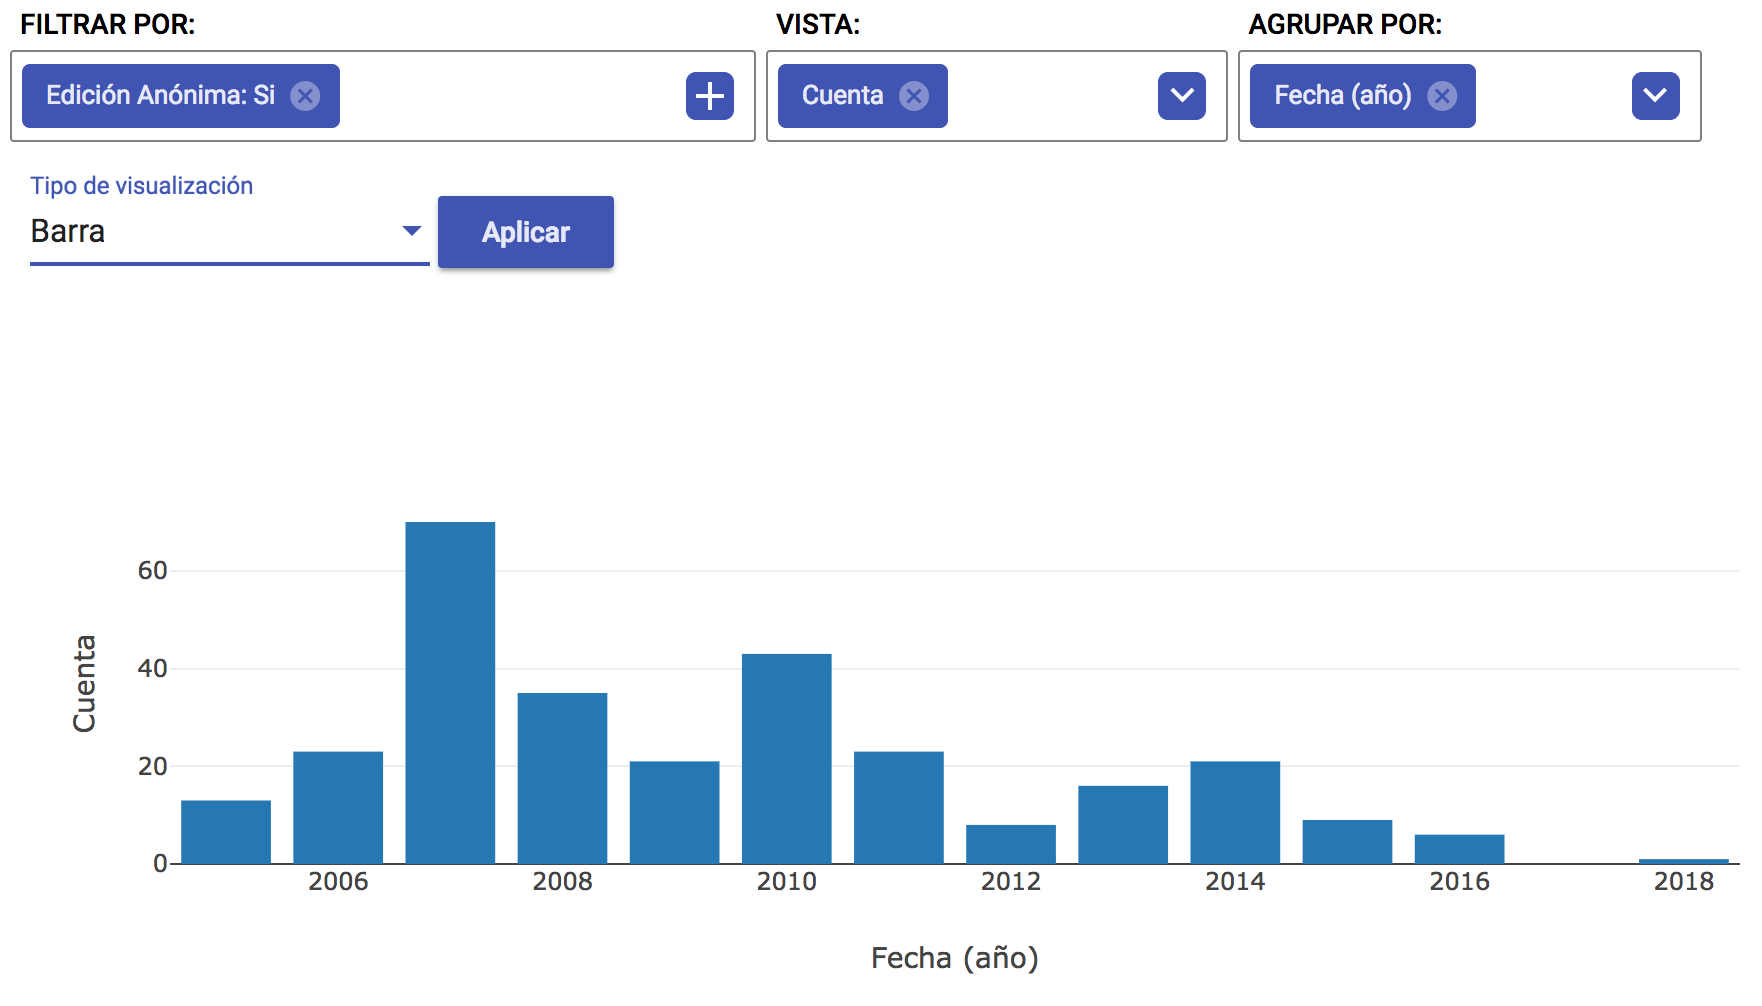
\includegraphics[scale=0.35]{images/marco_aplicativo/vis_bar.png}
          \captionof{figure}{Visualización tipo barra}
          \label{fig:vis_bar}
          \bigbreak
        \end{center}

    \item\textbf{Área}: gráfica similar a la de línea pero con el área pintada. Se puede observar en la \textbf{Figura \ref{fig:edit_vis}}.
    
    \item\textbf{Torta}: gráfica circular en donde los datos son representados por proporción, véase la \textbf{Figura \ref{fig:vis_pie}}.
        \begin{center}
          \bigbreak
          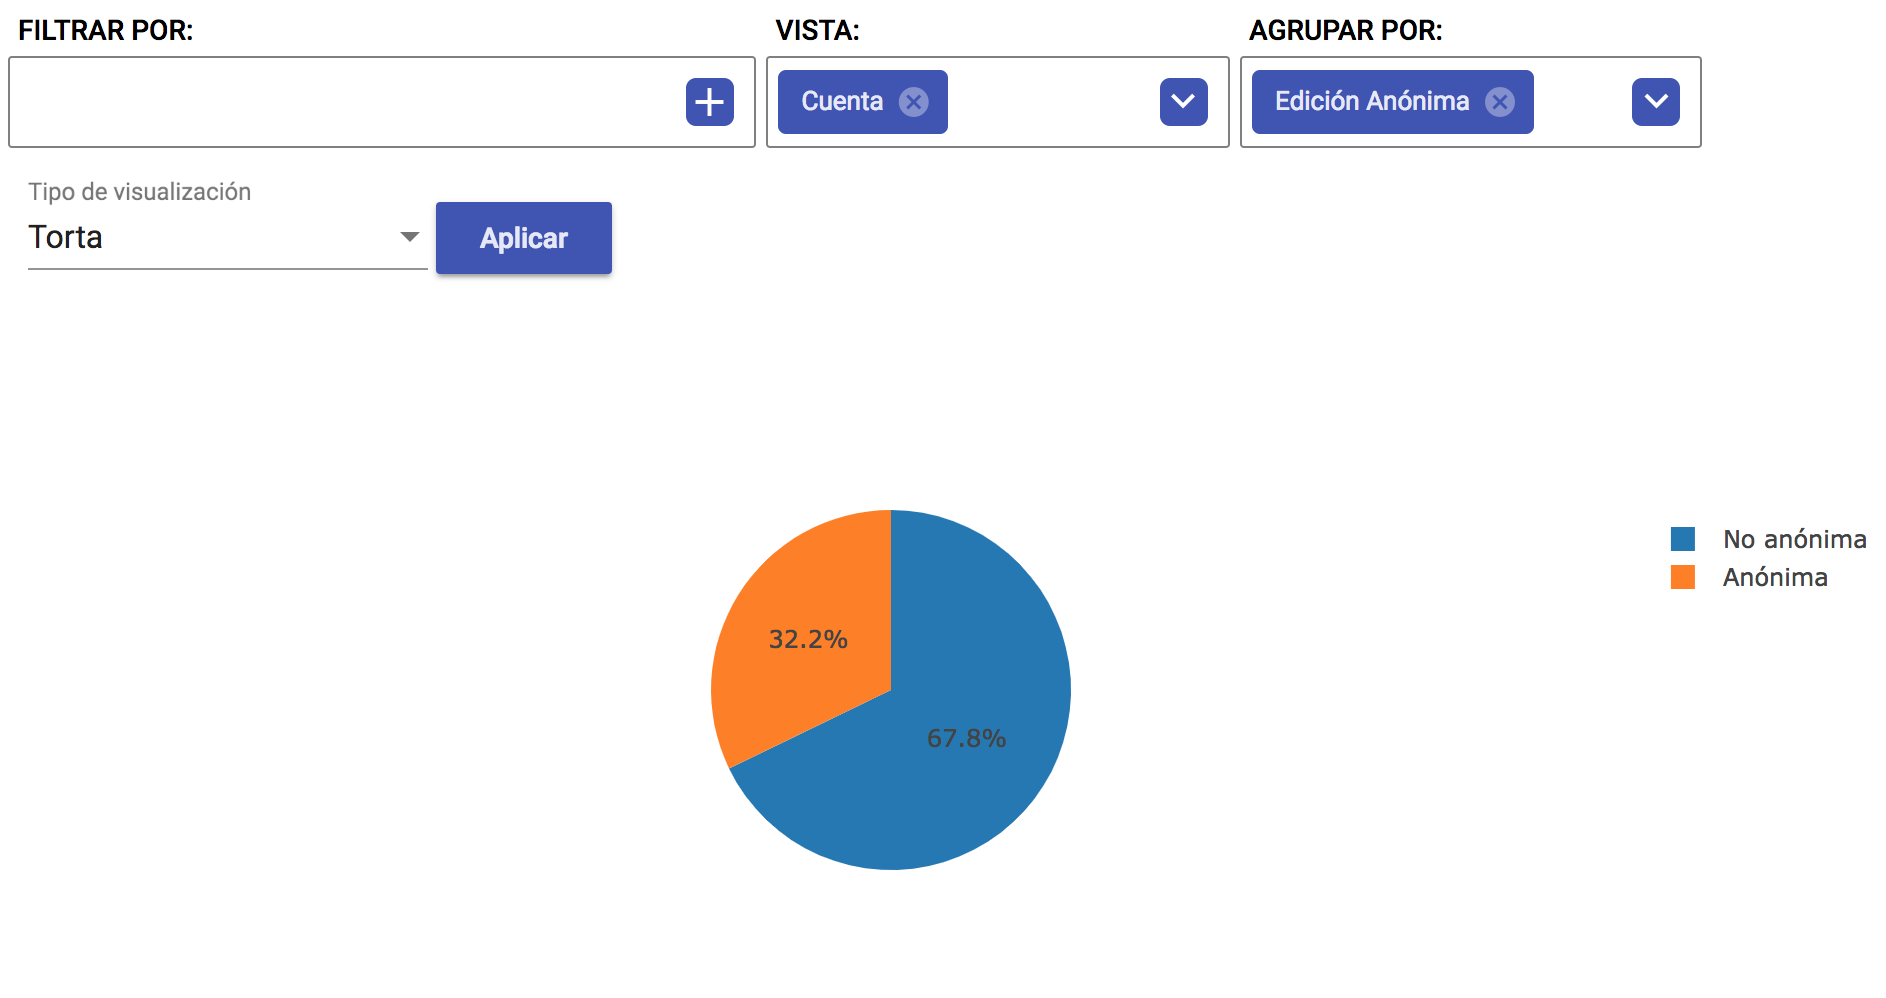
\includegraphics[scale=0.3]{images/marco_aplicativo/vis_pie.png}
          \captionof{figure}{Visualización tipo torta}
          \label{fig:vis_pie}
          \bigbreak
        \end{center}
        
    \item\textbf{Dispersión}: gráfica donde cada dato es representado por un punto, véase la \textbf{Figura \ref{fig:vis_scatter}}.
        \begin{center}
          \bigbreak
          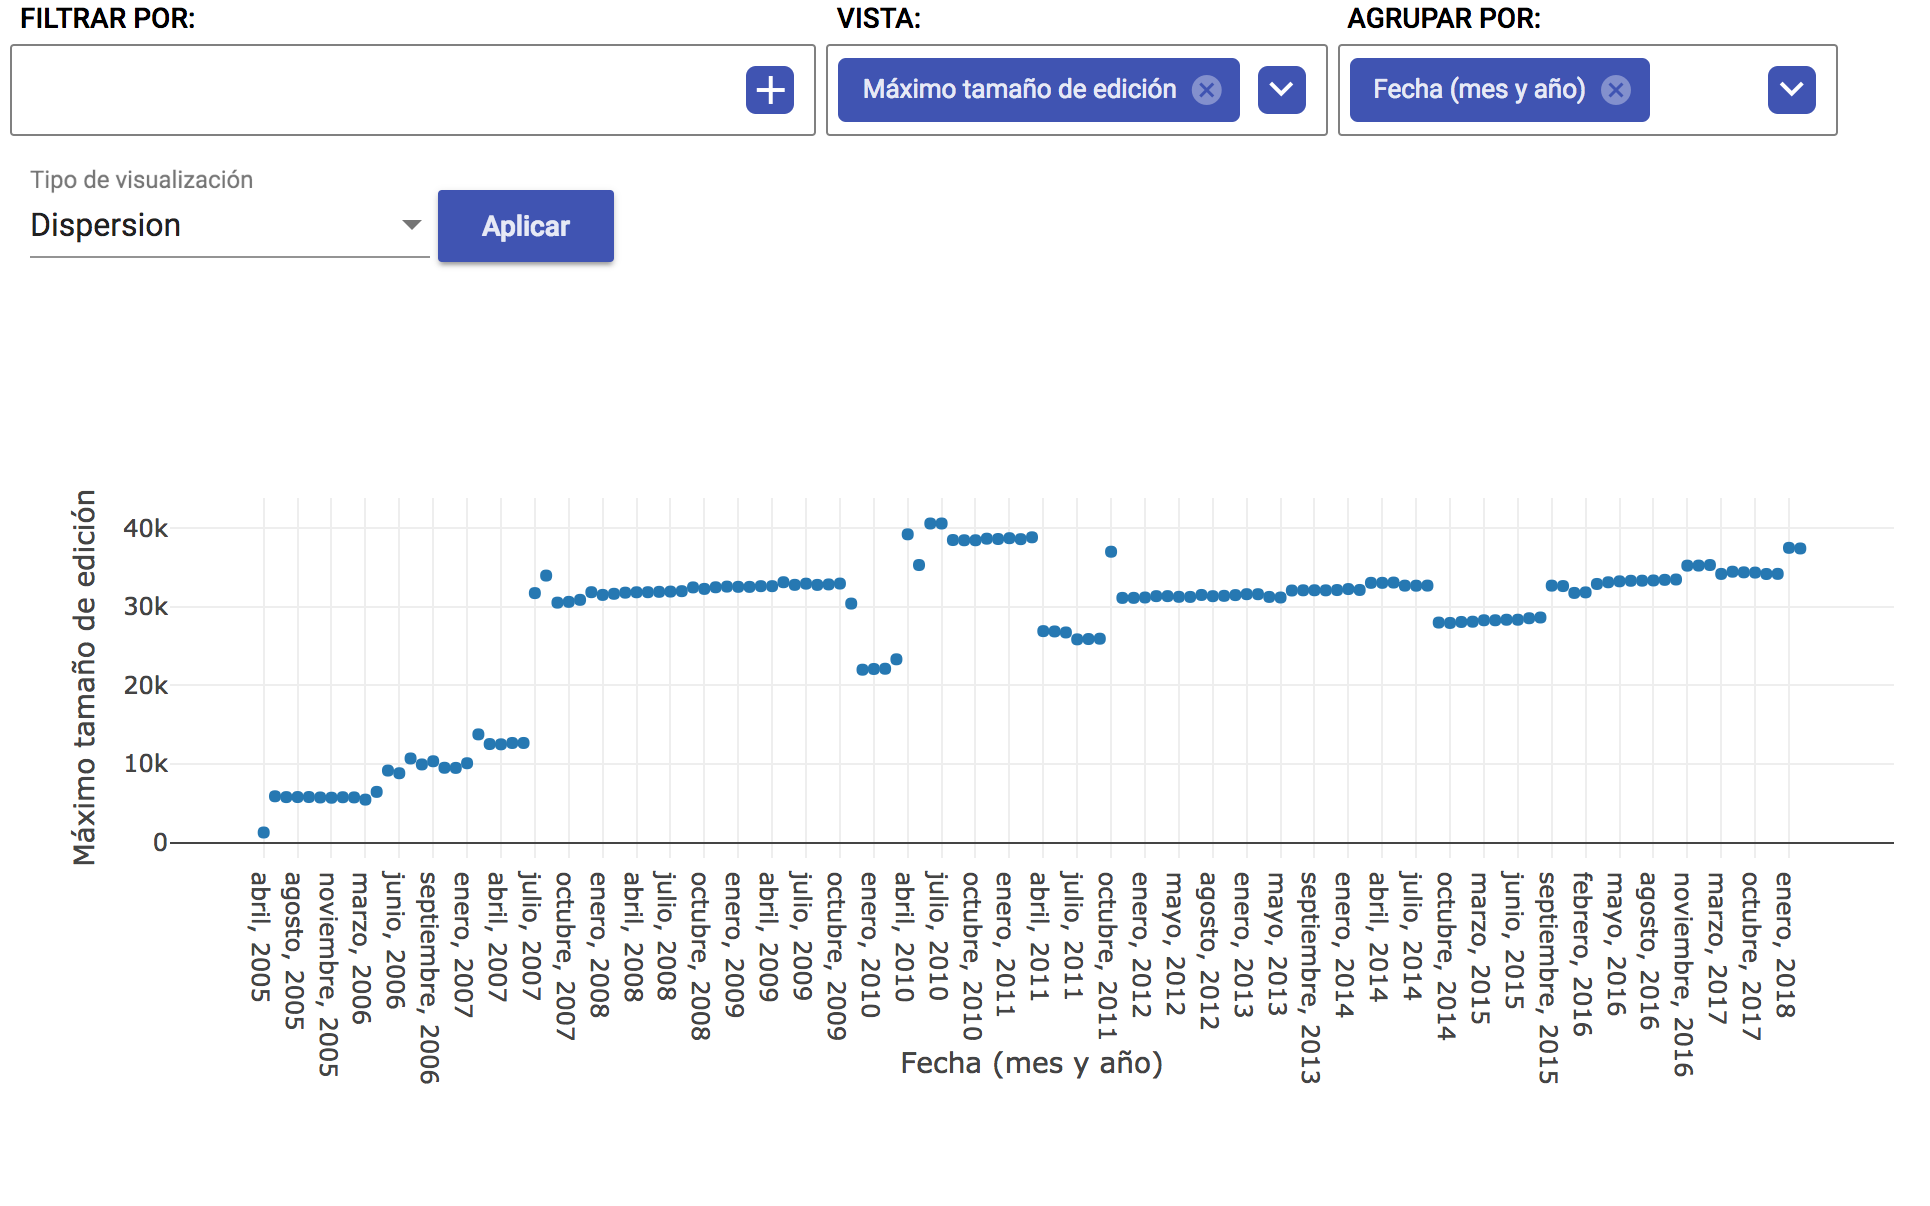
\includegraphics[scale=0.35]{images/marco_aplicativo/vis_scatter.png}
          \captionof{figure}{Visualización tipo dispersión}
          \label{fig:vis_scatter}
          \bigbreak
        \end{center}
  \end{itemize}
  
  \smallbreak
  \item\textbf{Implementar borrar artículo y visualización}
  \smallbreak
  
  Hasta ahora podemos crear artículos y visualizaciones, pero no borrar.
  
  Se implementaron las rutas en el API usando el método DELETE de HTTP para ambos recursos, cada servicio, el de visualizaciones y artículos encapsulando la petición. Por último, se habilitó la acción de eliminar en la interfaz para ambos casos.
  
  \smallbreak
  \item\textbf{Agregar zoom a gráfica del editor de visualizaciones}
  \smallbreak

  En el editor de visualizaciones puede que una visualización esté tan cargada de datos que la información se resuma y no se muestre toda, por lo que no será posible ver todos los datos.
  
  
  Plotly, automáticamente esconde la información para no sobrecargar la visualización, pero nos provee la funcionalidad de navegar en la visualización haciendo zoom.
  
  \begin{minted}[linenos]{ts}
  const layout = {
    xaxis: { title: this.chartXTitle, fixedrange: !this.chartZoom},
    yaxis: { title: this.chartYTitle, fixedrange: true},
  };
  \end{minted}
  
  La biblioteca permite pasarle un objeto con configuraciones al graficar. El atributo \textbf{xasis} hace referencia al eje 'x' y el atributo \textbf{yasis} al eje 'y'. Se habilitará el zoom en el eje 'x' solamente y se manejará con un input llamado \textbf{chartZoom}.
  
  \smallbreak
  \item\textbf{Agregar filtro de fecha en gráfica de Wiki History Flow}
  \smallbreak
  
  La gráfica Wiki History Flow suele ser muy pesada, en artículos con muchas ediciones puede tomarse un tiempo considerable en cargar debido a la petición de la información y el algoritmo para extraer la distancia del contenido.
  
  Como mecanismo para evitar larga espera, se implementó un filtro por rango de fecha, en donde se cargará solo las ediciones realizas en ese rango.
  
  En la primera carga se definió un rango de fecha que involucren las 200 primeras ediciones del artículo, véase la \textbf{Figura \ref{fig:date_range_wiki_history_flow}}.

  \begin{center}
    \bigbreak
    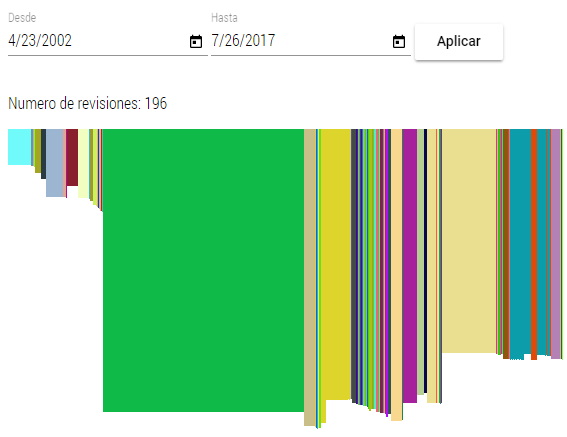
\includegraphics[scale=0.35]{images/marco_aplicativo/date_range_wiki_history_flow.png}
    \captionof{figure}{Wiki History Flow con filtro de rango de fecha.}
    \label{fig:date_range_wiki_history_flow}
    \bigbreak
  \end{center}
  
  \smallbreak
  \item\textbf{Agregar componente de \textit{preview} de visualización}
  \smallbreak

  Para poder observar una visualización es necesario entrar al detalle del artículo y seleccionar la que se quiere editar en el listado. Surge la necesidad de observar la gráfica de la visualización sin necesidad de acceder al editor.
  
  
  Se implementó una propiedad llamada \textit{preview}, donde cada elemento de la lista de visualizaciones proveerá la acción de habilitar o no el \textit{preview} de dicha visualización, véase la \textbf{Figura \ref{fig:toggle_preview}}.
  
  \begin{center}
    \bigbreak
    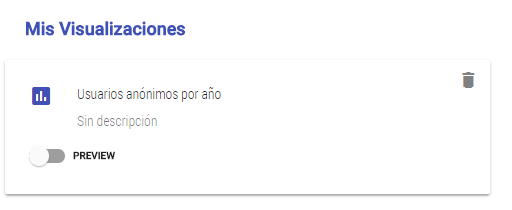
\includegraphics[scale=0.7]{images/marco_aplicativo/toggle_preview.png}
    \captionof{figure}{Toggle para habilitar/deshabilitar \textit{preview}.}
    \label{fig:toggle_preview}
    \bigbreak
  \end{center}
  
  Al habilitar el preview la gráfica de la visualización será mostrada en una sección del detalle de actividad haciendo uso del componente de visualización, observe la \textbf{Figura \ref{fig:preview_vis}}.
  
  \begin{center}
    \bigbreak
    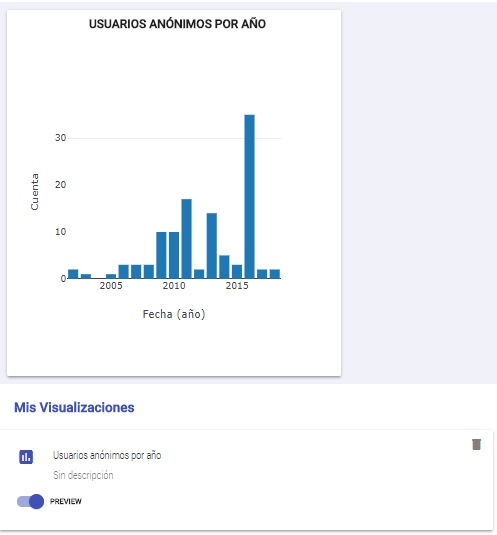
\includegraphics[scale=0.7]{images/marco_aplicativo/vis_preview.png}
    \captionof{figure}{Componente \textit{preview} de visualización en detalle de artículo.}
    \label{fig:preview_vis}
    \bigbreak
  \end{center}
  
  El \textit{preview} al ser pisado dirige al editor de la misma.
  
  \smallbreak
  \item\textbf{Incluir número de ediciones menores (con porcentaje) y número de editores en detalle de artículo}
  \smallbreak
  
  Se consideró agregar más información en el detalle del artículo, en donde el número de ediciones menores y número de editores pueden ser de utilidad.
  
  Apoyándose de la flexibilidad del API, para obtener el número de ediciones del artículo se envía el siguiente query:
  \begin{minted}[linenos]{json}
    [
      {
        "$match": {
          "title": "Programación dirigida por eventos",
          "locale": "es",
          "minor": {
            "$exists": true
          }
        }
      },
      {
        "$group": {
          "_id": null,
          "result": {
            "$sum": 1
          }
        }
      }
    ]
  \end{minted}
  
  Para obtener el número de editores se envía el siguiente query y se calcula el tamaño de la respuesta:
  \begin{minted}[linenos]{json}
    [
      {
        "$match": {
          "title": "Programación dirigida por eventos",
          "locale": "es"
        }
      },
      {
        "$group": {
          "_id": "$userid",
          "result": {
            "$sum": 1
          }
        }
      }
    ]
  \end{minted}
  
  \smallbreak
  \item\textbf{Definir e implementar gráficas generales en el detalle del artículo}
  \smallbreak
  
  Existen ciertas visualizaciones que seguramente sean de interés, por lo que se puede ofrecer de manera predeterminada y evitar que el usuario pierda tiempo en la creación de las mismas.
  
  En la lista de visualizaciones predeterminadas, en el detalle del artículo, se agregaron las siguientes visualizaciones: ediciones menores (\textbf{Figura \ref{fig:minor_edit}}), usuario anónimos (\textbf{Figura \ref{fig:anon_user}}), top 10 editores (\textbf{Figura \ref{fig:top_10}}) y número de ediciones por mes y año (\textbf{Figura \ref{fig:count_month_year}}.
  
  La información de estas visualizaciones se encuentran de manera estática en la versión actual dentro del código.
  
  Se implementó un componente capaz de visualizarlas en una vista nueva, similar al \textit{preview} y este fue el resultado:
  
  \begin{center}
    \bigbreak
    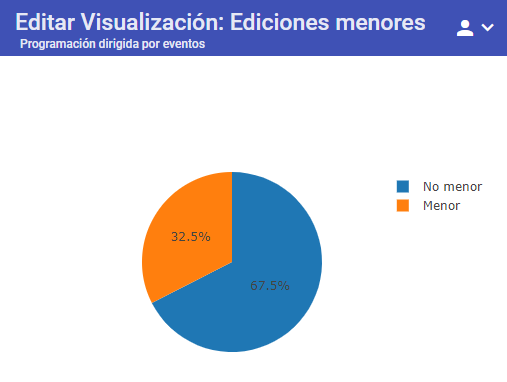
\includegraphics[scale=0.7]{images/marco_aplicativo/vis_default_minor_edit.png}
    \captionof{figure}{Visualización predefinida de total de ediciones menores vs. no menores del artículo 'Programación dirigida por eventos'}
    \label{fig:minor_edit}
    \bigbreak
  \end{center}
  
  \begin{center}
    \bigbreak
    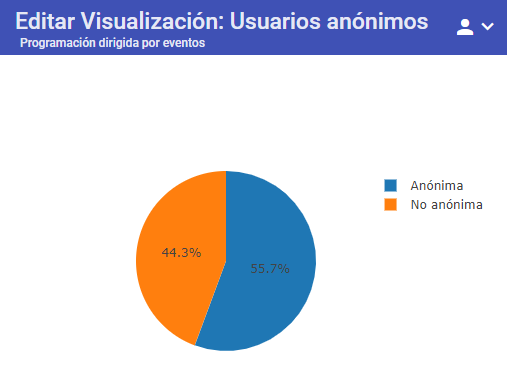
\includegraphics[scale=0.7]{images/marco_aplicativo/vis_default_anon_user.png}
    \captionof{figure}{Visualización predefinida de total de usuarios anónimos vs. no anónimos del artículo 'Programación dirigida por eventos'}
    \label{fig:anon_user}
    \bigbreak
  \end{center}

  \begin{center}
    \bigbreak
    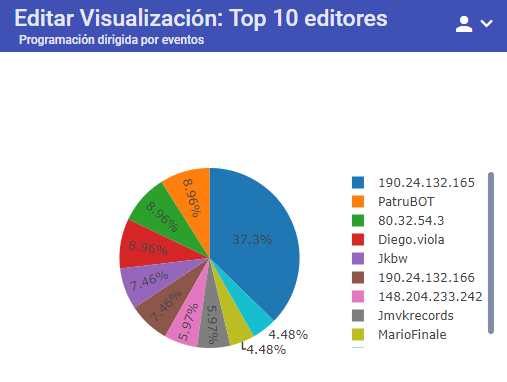
\includegraphics[scale=0.7]{images/marco_aplicativo/vis_default_top_10.png}
    \captionof{figure}{Visualización predefinida de Top 10 de usuarios con más ediciones del artículo 'Programación dirigida por eventos'}
    \label{fig:top_10}
    \bigbreak
  \end{center}

  \begin{center}
    \bigbreak
    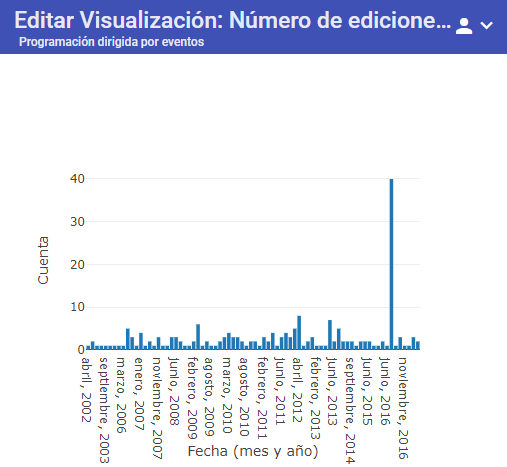
\includegraphics[scale=0.7]{images/marco_aplicativo/vis_default_count_month_year.png}
    \captionof{figure}{Visualización predefinida de total de ediciones agrupadas por mes y año del artículo 'Programación dirigida por eventos'}
    \label{fig:count_month_year}
    \bigbreak
  \end{center}
  
  

\end{enumerate}

\section{Arquitectura}
Anteriormente se había mencionado que la aplicación web está construida con el framework Angular, que hace uso de distintos servicios web: API de Wikimetrics, API de Usuarios y API de Wikipedia. Todo este ecosistema es indispensable para que la aplicación funcione correctamente, véase la \textbf{Figura \ref{fig:ecosytem_architecture}}.

\begin{center}
    \bigbreak
    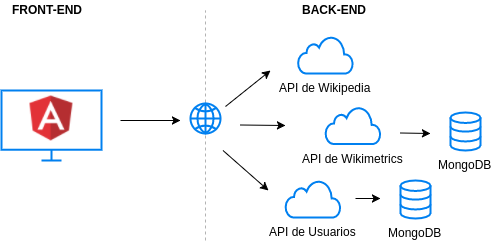
\includegraphics[scale=0.7]{images/marco_aplicativo/ecosystem.png}
    \captionof{figure}{Arquitectura general}
    \label{fig:ecosytem_architecture}
    \bigbreak
\end{center}

\subsection{Front-end}
Angular esta formado por una arquitectura basada en componentes, los componentes son piezas que conforman una vista. Algo importante en la arquitectura de Angular son los servicios, que son los encargados de proveer funcionalidades que no están relacionadas directamente con la vista. Para que los componentes puedan usar otros componentes y servicios es necesario contenerlos en un módulo. Los módulos permiten agrupar artefactos de Angular (incluyendo componentes y servicios) para que los componentes tengan el acceso a los mismos.

La aplicación desarrollada, tiene seis (6) componentes de ruta, que representan aquellos componentes que se \textit{renderizan} acorde a una ruta especificada en el navegador, véase la \textbf{Figura \ref{fig:tree_route_component}}. Cabe destacar que Angular necesita de un componente raíz que sea el encargado de encapsular los demás componentes, llamado \textbf{app-component}.


\begin{center}
    \bigbreak
    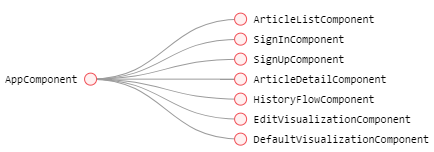
\includegraphics[scale=0.9]{images/marco_aplicativo/tree_route_component.png}
    \captionof{figure}{Componentes de ruta}
    \label{fig:tree_route_component}
    \bigbreak
\end{center}

Luego se tienen los otros componentes que son usados internamente en los componentes de ruta, en total tenemos los siguientes componentes:
\begin{minted}[linenos]{console}
article-card
article-detail (componente ruta)
article-list (componente ruta)
default-visualization (componente ruta)
edit-visualization (componente ruta)
history-flow (componente ruta)
loading
navbar
new-visualization
preview-visualization
query-selector
search-suggest
sign-in (componente ruta)
sign-up (componente ruta)
visualization

\end{minted}

A parte de los componentes propios, se usaron algunos componentes de Angular Material mencionados en ciertas tareas de la sección anterior.

Los componentes requieren el apoyo de los siguientes servicios:
\begin{minted}[linenos]{console}
article.service
auth-guard.service
auth.service
navbar.service
resize.service
visualization.service
wikimetrics.service
wikipedia.service
\end{minted}

Las dependencias del proyecto de angular se pueden encontrar en un archivo llamado \textbf{package.json} bajo el atributo \textit{dependencies}. Entre las dependencias se puede resaltar: D3, Luxon, Lodash y Text-diff. Cabe acotar que Plotly es una dependecia asíncrona que se descarga cuando el \textbf{index.html} se ejecuta por lo que no viene pre-cargada en el código de la aplicación.

\subsection{Back-end}
Para persistir la información de los usuarios es necesario implementar un servicio que provea y almacene los datos. De esta forma se implementó un servicio web RESTful, el cual trabaja en la existencia de recursos. Este servicio se construyó apoyándose del micro-framework Python Flask, que cubre las necesidades básicas, como recibir peticiones y manejar respuestas bajo los distintos métodos (GET, POST, PATCH y DELETE).

En el caso de este proyecto, se tuvieron que usar algunas extensiones de Flask para habilitar CORS y manejar autorización de recursos en la sesión con JWT.

Se implementaron las siguientes rutas en el API:
\begin{minted}[linenos]{console}
POST /sign-up
POST /sign-in
GET /articles
GET /articles/<locale>/<title>
POST /articles
PATCH /articles/<locale>/<title>/status/<status>
DELETE /articles/<locale>/<title>
POST /articles/<locale>/<title>/visualizations
PATCH /articles/<locale>/<title>/visualizations
DELETE /articles/<locale>/<title>/visualizations/<title_vis>
\end{minted}

Para persistir los datos se usó MongoDB, que es un manejador de sistema de base de datos no relacional. Al ser información única por usuario no era necesario relacionarla con la información de los otros usuarios, por lo que se trató cada usuario y configuración como un objeto separado en un documento JSON. La \textbf{Figura \ref{fig:db_model}} refleja el modelo de la base de datos.

\begin{center}
    \bigbreak
    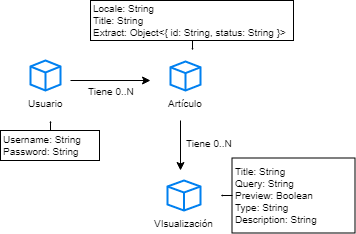
\includegraphics[scale=0.9]{images/marco_aplicativo/db_model.png}
    \captionof{figure}{Modelo de base de datos}
    \label{fig:db_model}
    \bigbreak
\end{center}

Un ejemplo de los datos crudos en MongoDB: 
\begin{minted}[linenos]{json}
{
    "user": {
        "username": "user1",
        "password": "106a6c241b8797f52e1e77317b96a201"
    },
    "articles": [
        {
            "locale": "en",
            "extract": {
                "status": "success",
                "id": "665d387e-e547-4275-8abf-1076eacf8f92"
            },
            "title": "Article 1",
            "visualizations": {
                "vis1": {
                    "query": "...",
                    "preview": true,
                    "type": "number",
                    "description": ""
                }
            }
        },
        {
            "locale": "en",
            "extract": {
                "status": "success",
                "id": "e7f48aa8-39e0-46c4-a23a-39485b65e0b4"
            },
            "title": "Article 2"
        }
    ]
}
\end{minted}

Se usó un driver llamado \textbf{PyMongo} para establecer la comunicación entre el código Python y la instancia de base de datos de MongoDB.





  
  

